% !TEX root = document.tex

\chapter{\label{chap:statix}WebDSL in Statix}

  In this chapter, we elaborate on the implementation of the WebDSL static semantics in Statix, using the examples from \cref{chap:webdsl} as a basis. We start this chapter by introducing the meta-DSL Statix. Once the goal and basics of Statix are stated, we describe the implementation of the type system that is the core of WebDSL. Next, we address and discuss the challenges faced while implementing non-trivial WebDSL features in Statix and lastly we reflect on the developer experience of using Statix to implement static analyses.

  \section{\label{sec:statix}Introduction to Statix}

    Statix is a constraint-based declarative language for the specification of type systems, introduced in 2018 \autocite{VanAntwerpen2018}. Since then, the meta-DSL Statix has become a part of the Spoofax Language Workbench and allows language developers to implement static analyses to provide language-specific feedback to developers on written code.

    A Statix specification consists of rules over terms that define constraints. Additionally, Statix rules build and query a \textit{scope graph} \autocite{Neron2015} that provides a language-agnostic representation of a program. A scope graph consists of nodes and edges that can be used to for example model the lexical scope of variables.

    \subsection{Language Signature}

      \begin{wrapfigure}{r}{0.58\linewidth}
        \vspace{-15pt}
        \capstart
        \begin{minted}[]{\statix}
  module x
  signature
    sorts
      Application
      Exp
    
    constructors
      Application : Exp       -> Application
      True        :              Exp
      False       :              Exp
      Int         : string    -> Exp
      Add         : Exp * Exp -> Exp
        \end{minted}
        \caption{\label{fig:statix-signatures}Language signature in Statix}
        \vspace{-10pt}
      \end{wrapfigure}

      Consider a language consisting of booleans, integers and addition, for which we want to create a type-checker with Statix. First, Statix requires us to declare all types and sorts that we will be using in the rules. These Statix constructor names have to match the constructors of the input term (the AST). The Statix code that declares the sorts and constructors of our example language is shown in \cref{fig:statix-signatures}. When writing a Statix specification for a language implemented in the Spoofax language workbench, it is a common practice to have the Statix signature generated from your SDF3 specification by the Statix signature generator (see \cref{subsec:statix-signature-generator}), to prevent code duplication.

      So far, our specification consists of two sorts. The \texttt{Application} sort defines the entry point of our language, it has one constructor with an identical name. Next, the sort \texttt{Exp} describes what expressions are allowed. It has four constructors: the Boolean values \texttt{True} and \texttt{False}, \texttt{Int} which requires an integer literal as subterm, and \texttt{Add} which takes two nested expressions as subterms. Examples of valid input according to our defined signature are shown in \cref{fig:statix-valid-input}.

      \begin{figure}[H]
        \begin{minted}[frame=single]{javascript}
  Application(True())                    // true
  Application(Int("42"))                 // 42
  Application(Add(Int("40"), Int("2")))  // 40 + 2
  Application(Add(Int("40"), False()))   // 40 + false
        \end{minted}
        \caption{\label{fig:statix-valid-input}Valid input terms for the described language}
      \end{figure}

    \subsection{Semantic Types}

      Not all of the valid input terms according to our signature are well-typed. For example, the last term shown in \cref{fig:statix-valid-input} features an addition of the integer literal \texttt{40} and the Boolean value \texttt{False}. Using Statix' constraint solving capabilities, we would like to give feedback to the programmer that the input is ill-typed.

      Given the code in \cref{fig:statix-signatures}, our Statix specification does not yet generate any constraints. Constraints that we would like to generate using Statix rules are firstly that a program must be well-typed and secondly, in order for an addition expression to be well-typed, its two subterms must be of integer type.

      \begin{wrapfigure}{r}{0.5\linewidth}
        \vspace{-20pt}
        \capstart
        \begin{minted}[]{\statix}
  module x
  signature
    sorts
      TYPE
    
    constructors
      BOOL : TYPE
      INT  : TYPE
        \end{minted}
        \caption{\label{fig:statix-type-signatures}Statix signature for Boolean and integer types}
        \vspace{-40pt}
      \end{wrapfigure}

      To reason about the types of expressions and use them in constraints, we must first define them in our specification, as shown in \cref{fig:statix-type-signatures}. To distinguish input sorts and constructors from semantic types that we will use in our constraints, those sorts and constructors are defined in upper-case. With the new \texttt{TYPE} sort that has two constructors: \texttt{BOOL} and \texttt{INT}, we can start generating constraints on input terms.

    \subsection{Predicates and Rules}

      \Cref{fig:statix-basic-rules} lists the Statix predicates and rules required to generate the constraints we want to be satisfied in order for a program to be well-typed. 

      \begin{figure}[H]
        \begin{minted}[]{\statix}
  module x
  rules

    applicationOk : Application
    applicationOk(Application(e)) :- { T }
      typeOfExp(e) == T.

    typeOfExp : Exp -> TYPE
    typeOfExp(True()) = BOOL().
    typeOfExp(False()) = BOOL().
    typeOfExp(Int(_)) = INT().
    typeOfExp(Add(e1, e2)) = INT() :-
      typeOfExp(e1) == INT(),
      typeOfExp(e2) == INT().
        \end{minted}
        \caption{\label{fig:statix-basic-rules}Statix predicates and rules for typing booleans, integers and addition}
      \end{figure}

      The type of all Statix predicates must be explicitly declared, for example the \texttt{applicationOk} predicate on \textbf{line 3} specifies that all rules of \texttt{applicationOk} match exactly one constructor \texttt{Application}. An instantiation of the \texttt{applicationOk} predicate is on \textbf{line 4}. In prose English it would read ``An application is well-typed, given that for some type \texttt{T}, the expression \texttt{e} has type \texttt{T}''.
      
      The other Statix rule in our small example specification is a \textit{functional predicate}, meaning that it returns a value. All but the last rules of the \texttt{typeOfExp} predicate compute a \texttt{TYPE} for a given expression, without conditions. The last rule of the example does have two conditions, in prose English it would read ``\texttt{e1} plus \texttt{e2} is of type \texttt{INT}, given that \texttt{e1} is of type \texttt{INT} and \texttt{e2} is of type \texttt{INT}''.

    \subsection{\label{subsec:building-and-querying-scope-graphs}Building and Querying Scope Graphs}

      When we expand our small example language with let-bindings and we want to add typing rules for this new construct, we come across a new feature in Statix. To facilitate typing rules for name binding, Statix uses \textit{scope graphs} \autocite{Neron2015}. Scope graphs are built out of three components: scopes, edges and declarations.

      \begin{figure}[h]
        \begin{subfigure}[b]{0.33\textwidth}
          \centering
          \begin{tikzpicture}
            \node (s_1) [scope] at(-1, 0) {s1};
            \node (x_1) [decl]  at(1, 0) {x};

            \draw[decl edge] (s_1.east) -- (x_1.west);
          \end{tikzpicture}
          \caption{\label{fig:scope-graph-example1}}
        \end{subfigure}
        \begin{subfigure}[b]{0.33\textwidth}
          \centering
          \begin{tikzpicture}
            \node (s_1) [scope]   at(-1, 0) {s1};
            \node (s_2) [scope]   at(-1, -2) {s2};
            \node (x_1) [decl]  at(1, 0) {x};
  
            \draw[scope edge] (s_2.north) -- (s_1.south) node[pos=0.5, xshift=-1ex] {P};
            \draw[decl edge] (s_1.east) -- (x_1.west);
          \end{tikzpicture}
          \caption{\label{fig:scope-graph-example2}}
        \end{subfigure}
        \begin{subfigure}[b]{0.33\textwidth}
          \centering
          \begin{tikzpicture}
            \node (s_1) [scope]   at(-1, 0) {s1};
            \node (s_2) [scope]   at(-1, -2) {s2};
            \node (x_1) [decl]  at(1, 0) {x};
            \node (y_1) [decl]  at(1, -1.5) {y};
            \node (z_1) [decl]  at(1, -2.5) {z};
  
            \draw[scope edge] (s_2.north) -- (s_1.south) node[pos=0.5, xshift=-1ex] {P};
            \draw[decl edge] (s_1.east) -- (x_1.west);
            \draw[decl edge] (s_2.east) -- (y_1.west);
            \draw[decl edge] (s_2.east) -- (z_1.west);
          \end{tikzpicture}
          \caption{\label{fig:scope-graph-example3}}
        \end{subfigure}
        \caption{\label{fig:scope-graph-examples}Scope graph examples}
      \end{figure}

      \Cref{fig:scope-graph-examples} showcases three examples of scope graphs. \Cref{fig:scope-graph-example1} consists of a single scope \texttt{s1} with declaration \texttt{x} that could be a model of a module with a single global variable \texttt{x} declared inside. The second example, \cref{fig:scope-graph-example2}, consists of two scopes: a root scope \texttt{s1} with again a declaration of \texttt{x}, and a scope \texttt{s2} with an outgoing edge to \texttt{s1} labeled \texttt{P}. The \texttt{P} label is often used to denote the relation of a lexical parent scope. In this example, \texttt{s2} could for example model an empty function declared in module \texttt{s1}. The last example again has two scopes, with one declaration in \texttt{s1} and two declarations in \texttt{s2}. This could model the same program as described previously, but now with two local variable declarations inside the function body of \texttt{s2}.

      \begin{wrapfigure}{r}{0.5\linewidth}
        \vspace{-20pt}
        \capstart
        \begin{minted}[]{\statix}
  module x
  signature
    constructors
      Let : string * Exp * Exp -> Exp
      Var : string             -> Exp

    name-resolution
      labels
        P // to denote parent scope

    relations
      var : string * TYPE
        \end{minted}
        \caption{\label{fig:statix-let-binding-signatures}Statix signature for let-bindings}
        % \vspace{-40pt}
      \end{wrapfigure}

      The first step in implementing let-bindings in Statix is adding the signature. In addition to the new constructors on \textbf{line 3 and 4}, we now introduce an edge label \texttt{P} and the relation \texttt{var}. The edge labels defined in the constructor provide the set of allowed labels to use in rules later on. The relation \texttt{var} on \textbf{line 11} specifies that any declaration made under the \texttt{var} relation in a scope, maps an identifier to its type.
      
      For illustration purposes, when we want to encode a single scope with two variable declarations, \texttt{x} of type \texttt{INT} and \texttt{b} of type \texttt{BOOL}, its scope graph would be as shown in \cref{fig:scope-graph-relations-example}.

      \begin{figure}[h]
        \centering
        \begin{tikzpicture}
          \node (s_1) [scope]   at(0, 0) {s1};
          \node (x_1) [decl]  at(3, 0.5) {x : INT()};
          \node (b_1) [decl]  at(3, -0.5) {b : BOOL()};

          \draw[decl edge] (s_1.east) -- (x_1.west) node[midway, sloped, fill=white] {var};
          \draw[decl edge] (s_1.east) -- (b_1.west) node[midway, sloped, fill=white] {var};
        \end{tikzpicture}
        \caption{\label{fig:scope-graph-relations-example}A scope graph containing a single scope with two declared variables}
      \end{figure}

      In Statix, scopes can be passed around as data. When we are evaluating an expression in our extended language, we now also want to pass the current scope. If the current input term that we are generating constraints for is a let-binding, we want to create a new scope, link it to the previous one, declare the variable in the new scope and evaluate the expression. To generate constraints for a variable expression, we want to query the scope graph and get its type. The Statix rules to reflect this are shown in \cref{fig:statix-let-binding-rules}.

      \begin{figure}[h]
        \begin{minted}[]{\statix}
  module x
  rules
    applicationOk : Application
    applicationOk(Application(e)) :- { s T }
      new s,
      typeOfExp(s, e) == T.

    typeOfExp : scope * Exp -> TYPE
    // ... previous rules
    typeOfExp(s, Let(x, e1, e2)) = T2 :- { s_let T1 }
      typeOfExp(s, e1) == T1,
      new s_let,
      s_let -P-> s,
      !var[x, T1] in s_let,
      T2 == typeOfExp(s_let, e2).

    typeOfExp(s, Var(x)) = T :-
      query var filter P*
                and { x' :- (x', _) == (x, _) }
                min $ < P
                and true
                in s |-> [(_, (_, T))].
        \end{minted}
        \caption{\label{fig:statix-let-binding-rules}Statix rules for let-bindings}
      \end{figure}

      \Cref{fig:statix-let-binding-rules} showcases various previously unexplained constructs:
      \begin{itemize}
        \item \textbf{Line 4} creates a new scope \texttt{s}. This scope is the root scope since it is created once at the start of an application and is not linked to any other scope.
        \item \textbf{Line 7} shows the new signature of the \texttt{typeOfExp} functional predicate. Given a scope and an expression, the rules of \texttt{typeOfExp} will compute the type of the expression.
        \item \textbf{Line 9-14} gives the typing rule of a let-binding. Given that the let-binding is of form \texttt{let x = e1 in e2}, the rule:
        \begin{itemize}
          \item computes the type of \texttt{e1} on line 10;
          \item creates a new scope \texttt{s\_let} on line 11 for the body of the let to evaluate in;
          \item declares variable \texttt{x} with associated type \texttt{T1} in the newly created scope \texttt{s\_let};
          \item computes the type of \texttt{e2} and this is the result of the rule.
        \end{itemize}
        \item \textbf{Line 16-21} holds the implementation of the variable typing rule. It executes a query with the following properties:
        \begin{itemize}
          \item It only returns entries in the \texttt{var} relation (line 17)
          \item It may follow zero or more \texttt{P} edge labels to other scopes (line 17);
          \item It only returns declarations under the same identifier as \texttt{x} (line 18);
          \item It prefers local declarations over declarations for which P edges must be followed (line 19);
          \item Shadowing according to the shadowing rules of line 19 is enabled (line 20);
          \item The query starts in the passed scope \texttt{s} (line 21);
          \item The result may only be one declaration (line 21).
        \end{itemize}
      \end{itemize}

      \Cref{fig:statix-let-binding-example} shows a possible input and the constructed scope graph after the constraints have been solved.

      \begin{figure}[h]
        \begin{subfigure}[b]{0.33\textwidth}
          \begin{minted}{javascript}
    let x = 1 in
      let y = x in
        x + y
          \end{minted}
          \caption{\label{fig:statix-let-binding-example-input}}
        \end{subfigure}
        \begin{subfigure}[b]{0.33\textwidth}
          \begin{minted}{javascript}
  Application(
    Let(
      "x", Int("1"), Let(
        "y", Var("x"), Add(
          Var("x"),
          Var("y")
        )
      )
    )
  )
          \end{minted}
          \caption{\label{fig:statix-let-binding-example-term}}
        \end{subfigure}
        \begin{subfigure}[b]{0.33\textwidth}
          \centering
          \begin{tikzpicture}
            \node (s_1) [scope]   at(-1, 0) {s1};
            \node (s_2) [scope]   at(-1, -2) {s2};
            \node (s_3) [scope]   at(-1, -4) {s2};
            \node (x_1) [decl]  at(2, -2) {x};
            \node (y_1) [decl]  at(2, -4) {y};
  
            \draw[scope edge] (s_2.north) -- (s_1.south) node[pos=0.5, xshift=-1ex] {P};
            \draw[scope edge] (s_3.north) -- (s_2.south) node[pos=0.5, xshift=-1ex] {P};
            \draw[decl edge] (s_2.east) -- (x_1.west) node[midway, sloped, fill=white] {var};
            \draw[decl edge] (s_3.east) -- (y_1.west) node[midway, sloped, fill=white] {var};
          \end{tikzpicture}
          \caption{\label{fig:statix-let-binding-example-sg}}
        \end{subfigure}
        \caption{\label{fig:statix-let-binding-example}Constructed scope graph after the example specification solved its contraints}
      \end{figure}

  \section{\label{sec:simple-type-systems}Encoding the WebDSL Basics}

  \begin{wrapfigure}{r}{0.5\linewidth}
    \vspace{-20pt}
    \capstart
    \begin{minted}[]{\statix}
  module x
  rules
    projectOk : scope
    unitOk    : scope * Unit
    sectionOk : scope * Section
    defOk     : scope * Definition
    typeOfExp : scope * Exp -> TYPE
    \end{minted}
    \caption{\label{fig:webdsl-basic-predicates}Predicates that form the basis of the WebDSL Statix specification}
    \vspace{-10pt}
  \end{wrapfigure}

      The WebDSL language adheres to a structure similar to many popular programming languages. A WebDSL application consists of multiple files. At the topmost level in a file, there is a module or \textit{unit} declaration. Within a module, multiple \textit{sections} of \textit{definitions} exist, such as pages, templates, entities and functions. A function consists of consecutive \textit{statements} such as variable assignment (\texttt{var n := 2}). At the innermost level, these statements contain \textit{expressions} that form the basis the WebDSL type system.

      To define well-typedness of the mentioned constructs, the Statix predicates as shown in \cref{fig:webdsl-basic-predicates} form the backbone of the WebDSL Statix specification.

    \subsection{\label{subsec:built-in-types-and-constants}Built-in Types and Constant Expressions}

      Constant expressions such as strings, integers and booleans form the building blocks of more complication constructs. For reasons explained later (see section \cref{subsec:built-in-extension}), a built-in type such as string is not declared as \texttt{STRING : TYPE} but instead as \texttt{BUILTINTYPE : scope * string -> TYPE}, where the instantiation of the string type is as follows: \texttt{BUILTINTYPE(s, "String")}.

      These built-in types are declared in a scope that is reachable from almost every location, the project scope, once per analysis. All WebDSL type declarations are made under the \texttt{type} relation, which associates the human readable type name with a \texttt{TYPE} term: \texttt{type : string * TYPE}. The part of the Statix specification to achieve this, and the resulting scope graph are shown in \cref{fig:webdsl-basics-built-in-types-decl}.

      \begin{figure}[h]
        \begin{subfigure}[b]{0.5\textwidth}
          \begin{minted}[firstline=3]{\statix}
module x
rules
  projectOk(s_project) :- 
    declareTypeBuiltIns(s_project).
    // ...

  declareTypeBuiltIns : scope
  declareTypeBuiltIns(s) :-
    declareType(s, "Int", 
      BUILTINTYPE(new, "Int")).
    // ...

  declareType : scope * string * TYPE
  declareType(s, name, t) :-
    !type[name, t] in s.
          \end{minted}
          \vspace{-10pt}
          \caption{\label{fig:webdsl-basics-built-in-types-decl-stx}}
        \end{subfigure}
        \begin{subfigure}[b]{0.5\textwidth}
          \centering
          \begin{tikzpicture}
            \node (s_1) [scope] at(0, 0) {s\_project};
            \node (t_1) [decl] at(0, -3) {Int : BUILTINTYPE(s\_int, "Int")};

            \draw[decl edge] (s_1.south) -- (t_1.north) node[midway, sloped, fill=white] {type};
          \end{tikzpicture}
          \caption{\label{fig:webdsl-basics-built-in-types-decl-sg}}
        \end{subfigure}
        \caption{\label{fig:webdsl-basics-built-in-types-decl}Declaring built-in types in the project scope}
      \end{figure}

      \begin{wrapfigure}{r}{0.57\textwidth}
        \capstart
        \begin{minted}[firstline=3]{\statix}
module x
rules
  typeOfExp(s, Const(Int(_))) = t :-
    resolveType(s, "Int") == [(_, (_, t))].

  resolveType : scope * string
    -> list((path * (string * TYPE)))
  resolveType(s, name) = ts :-
    query type filter P*
               and { t' :- t' == (name, _) }
               in s |-> ts.
        \end{minted}
        \caption{\label{fig:webdsl-basics-built-in-types-query}WebDSL integer constant expression typing rules}
      \end{wrapfigure}

      To retrieve a built-in type when evaluating a constant expression, we need to query the scope graph and resolve the type associated with the string representation. For example, the typing rules of an integer constant are listed in \cref{fig:webdsl-basics-built-in-types-query}. The integer typing rule introduces a constraint that the scope graph must contain a single type declaration associated with \texttt{"Int"} under the \texttt{type} relation. The result of the \texttt{resolveType} functional predicate on \textbf{line 2} should be a list containing one entry, namely the pair that we declared in \cref{fig:webdsl-basics-built-in-types-decl}. Other WebDSL constant expressions such as booleans, longs and floats have similar typing rules.

      \begin{wrapfigure}{r}{0.4\textwidth}
        \capstart
        \begin{minted}[frame=single, linenos, numbersep=-11pt]{javascript}
  "Hello world" // value
  "Hello ~( 1 + 2 )" // exp
  "Hello ~x.y" // simple exp
        \end{minted}
        \caption{\label{fig:statix-webdsl-string-interpolation-example}WebDSL string interpolation examples}
      \end{wrapfigure}

      The typing of perhaps the most common constant expression, a string, has an additional condition to be well-typed. Because string interpolation is possible, the constructor of a WebDSL string contains multiple parts that may impose additional constraints. A demonstration of the different interpolated parts is shown in \cref{fig:statix-webdsl-string-interpolation-example} and the complete typing rules are shown in \cref{fig:webdsl-basics-built-in-types-string}. The parts can be a simple string value which imposes no additional constraints, they can be a complete interpolated expression which requires the expression to be typed, or lastly they can be a ``simple'' expression which is directly inlineable.

      \begin{figure}
        \begin{minted}[firstline=3]{\statix}
module x
rules
  typeOfExp(s, Const(StringConst(String(str)))) = t :-
    resolveType(s, "String") == [(_, (_, t))],
    stringPartsOk(s, str).

  stringPartsOk maps stringPartOk(*, list(*))
  stringPartOk : scope * StringPart
  stringPartOk(s, StringValue(_)).
  stringPartOk(s, InterpExp(exp)) :- typed(s, exp).
  stringPartOk(s, InterpValue(InterpSimpleExp(simple_exp))) :- { T }
    typeOfSimpleExp(s, simple_exp) == T.
        \end{minted}
        \caption{\label{fig:webdsl-basics-built-in-types-string}WebDSL string typing rules}
      \end{figure}

      Now that all the typing rules for constants are implemented, typing rules for unary and binary operators are a step towards more complicated expressions. While it might seem trivial, we might require additional construct functional predicates for determining type compatibility or determining the resulting type of an expression.

    \subsection{\label{subsec:simple-variables}Variables}

      Similar to other imperative languages, WebDSL allows the use of variables to store values. These variables can be defined on multiple levels, such as in the module, within a function or at the top of a page/template definition. Additionally, functions may be embedded in entities, allowing direct access to entity properties as variables without having to prefix it with the \texttt{this} keyword.

      The basic variable declaration and resolving rules are shown in \cref{fig:webdsl-simple-variable-declaration-and-resolving}. Given a scope \texttt{s}, the declaration rule will make a declaration in \texttt{s} of variable \texttt{x} with associated type \texttt{t}.

      \begin{figure}[H]
        \begin{minted}[firstline=3]{\statix}
module x
rules
  declareVar : scope * string * TYPE
  declareVar(s, x, t) :-
    !var[x, t] in s,
    noDuplicateVarDefs(s, x)
      | error $[A variable named [x] already exists in this scope].

  resolveVar : scope * string -> list((path * (string * TYPE)))
  resolveVar(s, x) = ps :-
    query var filter P* /* We will explain the filter later in this section */
              and { x' :- x' == (x, _) }
              min $ < P /* We will explain the shadowing later in this section */
              and true
              in s |-> ps.
        \end{minted}
        \caption{\label{fig:webdsl-simple-variable-declaration-and-resolving}WebDSL variable declaration and resolving}
      \end{figure}

      \begin{wrapfigure}{r}{0.5\textwidth}
        \capstart
        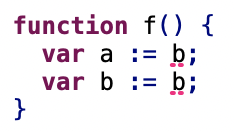
\includegraphics{../img/webdsl-simple-variable-declare-before-use}
        \caption{\label{fig:webdsl-simple-variable-declare-before-use}WebDSL requires declare-before-use of variables}
      \end{wrapfigure}

      The implementation of variable typing is similar to the example of let-bindings in \cref{subsec:building-and-querying-scope-graphs}. One difference between the let-bindings and WebDSL variables is that the introduction of consecutive statements in WebDSL requires a structure that defines declare-before-use semantics, to prevent backwards- or self-references such as shown in \cref{fig:webdsl-simple-variable-declare-before-use}.

      \Cref{fig:webdsl-simple-variable-declaration-scope} shows how the scope graph is constructed when there are consecutive statements. To catch declare-before-use related errors, a new scope is created for each statement (\textbf{line 6 and 7}). When constraints are generated for a constraint (such as on \textbf{line 11}), it has access to two scopes. Scope \texttt{s} denotes the scope of the current statement. Any scope graph queries will be executed in this scope. Example: the type of this statement is queried starting in scope \texttt{s} on \textbf{line 12}). Scope \texttt{s\_decl} denotes the scope of the next statement. Any scope graph declarations will be made this scope. Example: a variable declaration is being made in scope \texttt{s\_decl} on \textbf{line 14}).

      Using this tactic, a statement can never access declarations made by itself or by the next statements, it can only access declarations from previous statements.

      \begin{figure}
        \begin{minted}[firstline=3]{\statix}
module x
rules
  stmtOk : scope * scope * Statement

  stmtsOk : scope * list(Statement)
  stmtsOk(_, []).
  stmtsOk(s, [stmt | tail]) :- {s_decl s_next}
    new s_decl, s_decl -P-> s,
    new s_next, s_next -P-> s_decl,
    stmtOk(s, s_decl, stmt),
    stmtsOk(s_next, tail).

  stmtOk(s, s_decl, VarDecl(x, sort)) :- { t }
    t == typeOfSort(s, sort),
    inequalType(t, UNTYPED()) | error $[Unknown type [sort]] @sort,
    declareVar(s_decl, x, t),
    @x.type := t.  
        \end{minted}
        \caption{\label{fig:webdsl-simple-variable-declaration-scope}WebDSL statements use different scopes for querying and declaring data from the scope graph}
      \end{figure}

      An example of how this structure influences the building of scope graphs, a visualization of a function, accompanied by the scope graph of its body is shown in \cref{fig:webdsl-basics-declaration-scope-example}.

      \begin{figure}
        \begin{subfigure}[b]{0.3\textwidth}
          \begin{minted}[firstline=2]{\webdsl}
application test
  function f() : Int {
    var x := 1;
    var y := 2;
    return y;
  }
          \end{minted}
          \caption{\label{fig:webdsl-basics-declaration-scope-example-code}}
        \end{subfigure}
        \begin{subfigure}[b]{0.7\textwidth}
          \centering
          \begin{tikzpicture}
            \node (s_1) [scope]   at(-1, 0) {s1};
            \node (s_2) [scope]   at(-1, -2) {s2};
            \node (s_3) [scope]   at(-1, -4) {s2};
            \node (x_1) [decl]  at(4, -2) {x : BUILTINTYPE(s\_int, "Int")};
            \node (y_1) [decl]  at(4, -4) {y : BUILTINTYPE(s\_int, "Int")};
  
            \draw[scope edge] (s_2.north) -- (s_1.south) node[pos=0.5, xshift=-1ex] {P};
            \draw[scope edge] (s_3.north) -- (s_2.south) node[pos=0.5, xshift=-1ex] {P};
            \draw[decl edge] (s_2.east) -- (x_1.west) node[midway, sloped, fill=white] {var};
            \draw[decl edge] (s_3.east) -- (y_1.west) node[midway, sloped, fill=white] {var};
          \end{tikzpicture}
          \caption{\label{fig:webdsl-basics-declaration-scope-example-sg}}
        \end{subfigure}
        \caption{\label{fig:webdsl-basics-declaration-scope-example}Variable declarations example using a separate declaration scopes}
      \end{figure}

      Another difference between the let-binding rules from an earlier example and WebDSL variables is the complexity of the shadowing rules. The WebDSL variable shadowing rules which we reverse-engineered from the current compiler and static analysis implementation, state that the same variable identifier may be used multiple times, but never twice in the ``environment''. Such environments are: module scope, entity properties, functions, templates, etc. If a variable reference has multiple declarations in reach, the closest one according to the shadowing rules will be picked. The regular expression that defines the reachability of variables (left out in \textbf{line 9} of \cref{fig:webdsl-simple-variable-declaration-and-resolving}) is shown in \cref{fig:webdsl-simple-variable-well-formedness}.

      \begin{wrapfigure}{r}{0.5\textwidth}
        \begin{minted}[frame=single]{text}
    P*
    F*
    (
        (EXTEND? (INHERIT EXTEND?)*)
      | (DEF? (IMPORT | IMPORTLIB)?)
    )
        \end{minted}
        \caption{\label{fig:webdsl-simple-variable-well-formedness}Well-formedness predicate for variable paths}
      \end{wrapfigure}

      The edge label \texttt{P} as introduced in \cref{fig:webdsl-simple-variable-declaration-scope} is the edge label used for linking consecutive statements together. The other edge labels such as complicate this regular expression, and will be will be explained in more details in later sections when their use is discussed.

      \Cref{fig:webdsl-simple-variable-well-formedness} above defines what data is reachable from any point in the scope graph, but we also want some restrictions of declarations. The same environment such as function body or an entity definition may never declare the same variable twice. To achieve this, \textbf{line 4} of \cref{fig:webdsl-simple-variable-declaration-and-resolving} uses the helper predicate \texttt{noDuplicateVarDefs}. The implementation of this predicate is straight-forward and shown in \cref{fig:webdsl-simple-variable-no-duplicates}. The predicate queries the current scope and checks whether all scopes reachable using only \texttt{P} edge labels, results in a list containing only one entry.

      \begin{figure}
        \begin{minted}[firstline=3]{\statix}
module x
rules
  noDuplicateVarDefs : scope * string
  noDuplicateVarDefs(s, x) :-
    query var filter P*
              and { x' :- x' == (x, _) }
              in s |-> [_].
        \end{minted}
        \caption{\label{fig:webdsl-simple-variable-no-duplicates}The same variable identifier may only be declared once in an environment}
      \end{figure}

    \subsection{\label{subsec:type-compatibility}Type Compatibility}

      WebDSL has a notion of type compatiblity. For example, the WebDSL superclass of all entities is conveniently called \texttt{Entity}. When assigning a value to a variable that requires type \texttt{Entity}, passing an instance of a user-defined entity such as \texttt{Person} or \texttt{Project} also suffices. In this case, type \texttt{Person} is compatible with type \texttt{Entity}, but not the other way around. Type compatibility is not limited to entities. For instance, all WebDSL date types (\texttt{Date}, \texttt{Time}, \texttt{DateTime}) are compatible with each other. As a last example, null is compatible with many types. The examples given above are shown in \cref{fig:webdsl-basics-type-compatibility-example}.

      \begin{figure}
        \begin{minted}[firstline=2]{\webdsl}
application test
entity Person {}

function f() {
  var e : Entity := Person{}; // all user-defined entities are compatible with Entity
  var d : Date := now(); // now() produces a value of type DateTime
  var p : Person := null; // null is compatible with many types
}
        \end{minted}
        \caption{\label{fig:webdsl-basics-type-compatibility-example}Examples of type compatibility in WebDSL}
      \end{figure}

      To encode the type compatibility as shown in \cref{fig:webdsl-basics-type-compatibility-example} in Statix, we need a predicate that tells us, given two types \textit{A} and \textit{B}, if type \textit{A} is compatible with with \textit{B}. The signature and its general rules are shown in \cref{fig:type-compatibility-statix-basic}.

      \begin{figure}
        \begin{minted}[firstline=3]{\statix}
          module x
          rules
  typeCompatible : TYPE * TYPE
  // By default, two types are not compatible
  typeCompatible(T1, T2).
  // Same type is always compatible
  typeCompatible(T, T).
        \end{minted}
        \caption{\label{fig:type-compatibility-statix-basic}WebDSL type compatibility predicate and general rules}
      \end{figure}

      With only the basic rules from \cref{fig:type-compatibility-statix-basic}, we have created the equality (\texttt{==}) from Statix in predicate form. The advantage of listing it like this, is that we can now add rules to make it fit the WebDSL type system. To continue the example of \texttt{null} being compatible with every type, we can add the rules shown in \cref{fig:null-type-compatibility} to achieve this. An example of how to use our new \texttt{typeCompatible} predicate is also given on \textbf{line 8} of \cref{fig:null-type-compatibility}.

      \begin{figure}
        \begin{minted}[firstline=3]{\statix}
          module x
          rules
  typeOfExp(_, Null()) = NULL().
  typeCompatible(NULL(), _).

  // example of usage:
  stmtOk(s, VarDeclInit(x, sort, exp), _) :- { sortType expType }
    sortType == typeOfSort(s, sort),
    expType == typeOfExp(s, exp),
    typeCompatible(expType, sortType)
      | error $[Expression [exp] is not of type [sort], got type [expType]] @exp,
    declareVar(s, x, sort),
    @x.type := t.
        \end{minted}
        \caption{\label{fig:null-type-compatibility}Compatibility of the null expression encoded in Statix}
      \end{figure}

      \begin{itemize}
        \item [\textbf{TO-DO:}]
        \item Add (plus) LUB
      \end{itemize}

    \subsection{\label{subsec:boolean-logic}Boolean Logic in Statix}

      \begin{itemize}
        \item [\textbf{TO-DO:}]
        \item Show sort and constructors
        \item Examples of where it's necessary
      \end{itemize}

    \subsection{\label{subsec:simple-entities}Entities and Properties}

      Entities form the basis of the type system and data structure in a WebDSL application. Using Hibernate as an object-relational mapping (ORM) tool, instances of entities can be persisted without explicit communication with a database management system. Entities typically have multiple properties which values are persisted, and functions that can be called and will be executed in the scope of the instantiated entity. Entity properties and entity functions together form the entity body declarations.

      In the WebDSL type system, entities are declared in the scope of the module they are defined in. An entity is a type in the WebDSL type system, similar to built-in types such as \texttt{String} and \texttt{Int}. The Statix code to declare entities is shown in \cref{fig:webdsl-entity-declaration-statix} and an example of a simple program with entity definition plus its scope graph is shown in \cref{fig:webdsl-entity-example}.

      \begin{figure}
        \begin{minted}[firstline=2]{\statix}
module x
  signature
    constructors
      // an entity constructor has two subterms:
      // - the entity name
      // - the scope of the entity where all the properties and 
      //   functions are declared
      ENTITY : string * scope -> TYPE

  rules
    defOk(s_module, EntityNoSuper(entity_name, body)) :- { s_entity }
      // a new scope for the entity is created and linked to the module scope
      // using the `DEF' (for definition) edge label
      new s_entity, s_entity -DEF-> s_module,

      // the new entity is declared as type in the module scope
      declareType(s_module, entity_name, ENTITY(entity_name, s_entity)),

      // finally a helper rule is called that properly handles
      // the entity body definitions (properties, functions, etc.)
      declEntityBody(s_entity, entity_name, body).
        \end{minted}
        \caption{\label{fig:webdsl-entity-declaration-statix}The Statix rules for declaring entities}
      \end{figure}

      \begin{figure}
        \begin{subfigure}[b]{0.2\textwidth}
          \begin{minted}[firstline=1]{\webdsl}
  module m
    entity Person { 
      // no properties
      // for now...
    }
          \end{minted}
          \caption{\label{fig:webdsl-entity-example-webdsl}}
        \end{subfigure}
        \begin{subfigure}[b]{0.8\textwidth}
          \centering
          \begin{tikzpicture}
            \node (s_m) [scope]   at(-1, 0) {s\_m};
            \node (s_p) [scope]   at(-1, -2) {s\_person};
            \node (t_p) [decl]  at(4.5, 0) {Person : ENTITY("Person", s\_person)};
  
            \draw[scope edge] (s_p.north) -- (s_m.south) node[pos=0.5, xshift=2ex] {DEF};
            \draw[decl edge] (s_m.east) -- (t_p.west) node[midway, sloped, fill=white] {type};
          \end{tikzpicture}
          \caption{\label{fig:webdsl-entity-example-sg}}
        \end{subfigure}
        \caption{\label{fig:webdsl-entity-example}An example of entity definition in WebDSL}
      \end{figure}

      The \texttt{declareType} and \texttt{resolveType} rules as introduced in \cref{fig:webdsl-basics-built-in-types-decl} need to be updated to work as intended for resolving and declaring entities. To prevent duplicate entity definitions, the \texttt{declareType} rule is extended with one additional rule as shown in \cref{fig:webdsl-entity-new-type-declare-and-resolve}. \textbf{Line 4} was added to \texttt{declareType}, to make sure when you declare a new type or entity, its name is unique.

      \begin{figure}
        \begin{minted}[firstline=3]{\statix}
module x
  rules
    declareType : scope * string * TYPE
    declareType(s, name, t) :-
      !type[name, t] in s,
      resolveType(s, name) == [(_, (_, t))]
        | error $[Type [name] is defined multiple times] @name.

    resolveType : scope * string -> list((path * (string * TYPE)))
    resolveType(s, name) = typesOf(ts) :-
      query type filter P* DEF?   // resolving a type may
                                  // optionally follow DEF edge label
                 and { t' :- t' == (name, _) }
                 in s |-> ts.
        \end{minted}
        \caption{\label{fig:webdsl-entity-new-type-declare-and-resolve}\texttt{declareType} now shows an error when two types with the same name are declared and \texttt{resolveType} may optinally follow a \texttt{DEF} edge label}
      \end{figure}

      In addition to the added constraint to the \texttt{declareType} rule, we added an optional \texttt{DEF} edge label that may be followed when querying the scope graph for a type (\textbf{{line 9}} of \cref{fig:webdsl-entity-new-type-declare-and-resolve}). The \texttt{DEF} (short for defintion) is used to link the scope of top-level elements, such as entities and functions, to the module scope. This can be seen in \textbf{line 13} of \cref{fig:webdsl-entity-declaration-statix}.

      So far, there has been no reason to query for types inside the entity body because we have always worked with empty entities. In practice, entities are filled with properties and functions. \textbf{Line 20} of \cref{fig:webdsl-entity-declaration-statix} calls the \texttt{declEntityBody} predicate, of which the implementation is shown in \cref{fig:webdsl-entity-body-declaration} and an example of an entity definition with two properties is shown in \cref{fig:webdsl-entity-body-example}.
      
      Entity properties are declared under the variable relation inside the entity scope, such that functions inside entities can reference their own properties without using the \texttt{this} prefix. The \texttt{this} construct is supported, but not necessary. Declaring properties in this way, allows us to reuse the already existing rules such as those against duplicate definition, without duplicating the code for another relation.

      \begin{figure}
        \begin{minted}[firstline=3]{\statix}
module x
  rules
  declEntityBody maps declEntityBodyDeclaration(*, *, list(*))
  declEntityBodyDeclaration : scope * string * EntityBodyDeclaration

  // entity property
  declEntityBodyDeclaration(s, ent, 
      Property(x, propkind, sort, PropAnnos(annos))) :- { sortType }

    // resolve the type of the property
    sortType == typeOfSort(s, sort),

    // there are some restrictions on property types
    sortType != UNTYPED()
      | error $[Cannot resolve type [sort]] @sort,
    sortType != VOID()
      | error $[Property type 'Void' not allowed] @sort,
    sortType != REF(_)
      | error $[Reference type is not allowed in property] @sort,
    isValidTypeForPropKind(propkind, sort, sortType),

    // declare the property as variable in the entity scope
    declareVar(s, x, sortType),

    // use a helper predicate to check for the uniqueness of
    // the property name
    resolveLocalProperty(s, x) == [_]
      | error $[Property [x] of entity [ent] is defined multiple times] @x.
        \end{minted}
        \caption{\label{fig:webdsl-entity-body-declaration}Statix rules for declaring the entity body}
      \end{figure}

      \begin{figure}
        \begin{subfigure}[b]{0.3\textwidth}
          \begin{minted}[firstline=1]{\webdsl}
  module m
    entity Person { 
      name        : String
      dateOfBirth : Date
    }
          \end{minted}
          \caption{\label{fig:webdsl-entity-body-example-webdsl}}
        \end{subfigure}
        \begin{subfigure}[b]{0.7\textwidth}
          \centering
          \begin{tikzpicture}
            \node (s_m) [scope]   at(-1, 0) {s\_m};
            \node (s_p) [scope]   at(-1, -2) {s\_person};
            \node (t_p) [decl]  at(4.5, 0) {Person : ENTITY("Person", s\_person)};
            \node (name) [decl]  at(5.5, -1.5) {name : BUILTINTYPE(s\_string, "String")};
            \node (dob) [decl]  at(5.5, -2.5) {dateOfBirth : BUILTINTYPE(s\_date, "Date")};
  
            \draw[scope edge] (s_p.north) -- (s_m.south) node[pos=0.5, xshift=2ex] {DEF};
            \draw[decl edge] (s_m.east) -- (t_p.west) node[midway, sloped, fill=white] {type};
            \draw[decl edge] (s_p.east) -- (name.west) node[midway, sloped, fill=white] {var};
            \draw[decl edge] (s_p.east) -- (dob.west) node[midway, sloped, fill=white] {var};
          \end{tikzpicture}
          \caption{\label{fig:webdsl-entity-body-example-sg}}
        \end{subfigure}
        \caption{\label{fig:webdsl-entity-body-example}An example of an entity definition with multiple properties}
      \end{figure}

      \begin{itemize}
        \item [\textbf{TO-DO:}]
        \item Instantiation
      \end{itemize}

    \subsection{\label{subsec:simple-functions}Functions}

      \begin{itemize}
        \item [\textbf{TO-DO:}]
        \item Declaration and resolving
        \item Prevent duplicates
        \item Parameters
      \end{itemize}

    \subsection{\label{subsec:simple-pages}Pages and Templates}

      The user-inferface of a WebDSL application is built out of \textit{pages} and \textit{templates}. A page defines a path that is able to be requested by the browser while a template is a reusable component that can be part of a page or nested in other templates.

      \begin{figure}
        \begin{minted}[firstline=2]{\statix}
module x
  signature
    constructors
      PAGE     : string * list(TYPE) -> TYPE
      TEMPLATE : string * list(TYPE) -> TYPE

    relations
      page     : string * TYPE
      template : string * TYPE
        \end{minted}
        \caption{\label{fig:statix-page-and-template-constructors}Statix signature for pages and templates}
      \end{figure}

      The name of a page must be unique, while a template can be defined multiple times for different argument types (\textit{overloading}), but never multiple times for the same argument types. Page and template definitions must be declared in the scope graph such that they can be referenced or checked for uniqueness. The statix rules to implement these checks can be found in \cref{fig:webdsl-page-and-template-definition}.

      \begin{figure}
        \begin{minted}[firstline=3]{\statix}
module x
  rules
  declarePage : scope * string * list(TYPE)
  declarePage(s, p, ts) :-
    !page[p, PAGE(p, ts)] in s,
    resolveTemplate(s, p) == []
      | error $[Multiple page/template definitions with name [p]] @p,
    resolvePage(s, p) == [_]
      | error $[Multiple page/template definitions with name [p]] @p.

  declareTemplate : scope * string * list(TYPE)
  declareTemplate(s, t, ts) :-
    !template[t, TEMPLATE(t, ts)] in s,
    resolvePage(s, t) == []
      | error $[Multiple page/template definitions with name [t]] @t,
    filterTemplateResultsArgs(resolveTemplate(s, t), ts) == [_]
      | error $[Multiple page/template definitions with name [t] and argument types [ts]] @t.
        \end{minted}
        \caption{\label{fig:webdsl-page-and-template-definition}Statix rules for declaring WebDSL pages and templates}
      \end{figure}

      \begin{itemize}
        \item [\textbf{TO-DO:}]
        \item Show code and resulting scope graph with a page and a template
      \end{itemize}

      Type-checking a page reference is easier than the that of a template, since a page definition cannot be overloaded. In order for a page reference to be well-typed, the page must be defined exactly once, and the types of the passed arguments must be compatible with the parameter types of the page. The Statix rules that ticks those boxes is shown in \cref{fig:webdsl-page-type-checking}.

      \begin{figure}
        \begin{minted}[firstline=3]{\statix}
module x
rules
  pageCallOk : scope * string * list(Exp)
  pageCallOk(s, p, args) :- {argTypes ts}
    pageType(s, p) == PAGE(_, ts)
      | error $[There is no page with signature [p]] @p,
    argTypes == typesOfExps(s, args),
    typesCompatible(argTypes, ts)
      | error $[Given argument types not compatible with page definition] @args.
    
  // root page is always accessible from all locations
  pageCallOk(_, "root", []).
        \end{minted}
        \caption{\label{fig:webdsl-page-type-checking}Statix rules for type-checking a page reference}
      \end{figure}

      \begin{itemize}
        \item [\textbf{TO-DO:}]
        \item Explain resolving templates later
        \item Ajax templates
        \item Template elements
      \end{itemize}

      \subsection{\label{subsec:access-control}Access Control}

      \begin{itemize}
        \item [\textbf{TO-DO:}]
        \item Principal
        \item References to pages and templates
        \item Wildcards
        \item Pointcuts?
      \end{itemize}

  \section{\label{sec:inheritance}Inheritance}

    \subsubsection{Linking the Scopes}
      The implementation of inheritance requires the scope of the sub- and super-entity to be connected such that Statix queries can resolve to declarations from the super-entity when necessary. To achieve this, we introduce an edge label \texttt{INHERIT} as shown in listing \emph{TO-DO}.
      \begin{minted}[firstline=3]{\statix}
  module x
  signature
    name-resolution
      labels
        INHERIT // inherit edge label for subclasses
      \end{minted}
      Declarations of sub-entities will generate constraints as shown in listing \emph{TO-DO}.
      \begin{minted}[firstline=3]{\statix}
  module x
  rules
    defOk(s_global, Entity(x, super, bodydecs)) :- {s_entity super' s_super}
      resolveEntity(s_global, super) == [(_, (super', ENTITY(s_super)))],
      new s_entity, s_entity -INHERIT-> s_super,
      noCircularInheritance(s_entity),
      declEntity(s_global, s_entity, x, bodydecs),
      @super.ref := super'.
      \end{minted}
      First of all, the super-entity refered to in the declaration must refer to an existing entity in the scope graph. Secondly, the new scope belonging to the sub-entity \texttt{s\_entity} is linked to the scope of the super class \texttt{s\_super} via an \texttt{INHERIT} edge. Finally, some additional constraints are generated to make sure no circular inheritance exists and constraints for the entity body declarations of the sub-entity are generated.

      Previously, the resolving of variables was done using the query as shown in listing \emph{TO-DO}
      \begin{minted}[firstline=3]{\statix}
  module x
  rules
    resolveVar(s, x) = ps :-
      query var filter P* F* IMPORT*
                and { x' :- x' == (x, _) }
                min $ < P, P < F, F < IMPORT
                and true
                in s |-> ps.
      \end{minted}
      The new query in listing \emph{TO-DO} reflects the addition of the \texttt{EXTEND} label. The addition of \texttt{INHERIT*} in the query filter makes all variables declared in ancestors reachable.
      \begin{minted}[firstline=3]{\statix}
  module x
  rules
    resolveVar(s, x) = ps :-
      query var filter P* F* INHERIT* IMPORT*
                and { x' :- x' == (x, _) }
                min $ < P, P < F, F < INHERIT, INHERIT < IMPORT
                and true
                in s |-> ps.
      \end{minted}

    \subsubsection{Overwriting Functions}
      Generally, overwriting functions is not allowed in WebDSL. Entity functions are an exception to this such that entity function definitions shadow global function definitions. With the introduction of inheritance there comes another exception, namely that sub-entities are allowed to overwrite function definitions of their ancestors.

      Previously, the resolving of entity functions was done using the query as shown in listing \emph{TO-DO} below.

      \begin{minted}[firstline=3]{\statix}
  module x
  rules
    resolveEntityFunction(s, x) = ps :-
      query function filter e
                      and { x' :- x' == (x, _) }
                      min
                      in s |-> ps.
      \end{minted}

      With the introduction of entity inheritance, the path well-formedness over edge labels should be tweaked such that functions from ancestors are in scope. Changing \texttt{filter e} to \texttt{filter INHERIT*} accomplishes this. The resulting query is in listing \emph{TO-DO} below.

      \begin{minted}[firstline=3]{\statix}
  module x
  rules
    resolveEntityFunction(s, x) = ps :-
      query function filter INHERIT*
                      and { x' :- x' == (x, _) }
                      min /* */
                      in s |-> ps.
      \end{minted}

      This query definition works perfectly when sub-entities do not overwrite functions. When a sub-entity does define a function that is already defined in one of its ancestors, resolving the entity function gives two results while we would like only one result, namely the overwritten function defined in the sub-entity. To tackle this challenge, we defined a Statix anonymous shadowing rule combined with a label order. This ensures that when two functions with the same name and argument types exist, only the most specific (i.e. the least inheritance edges) is returned. This is implemented as shown in listing \emph{TO-DO}.

      \begin{minted}[firstline=3]{\statix}
  module x
  rules
    resolveEntityFunction(s, x) = ps :-
      query function filter INHERIT*
                      and { x' :- x' == (x, _) }
                      /* prioritize local scope over inheritance */
                      min $ < INHERIT
                      /* shadow when function name and argument types match */
                      and {
                      (f, FUNCTION(args, _, _)),
                      (f, FUNCTION(args, _, _))
                      }
                      in s |-> ps.
      \end{minted}

    \subsubsection{Entity Type Compatibility}
      A great perk of having inheritance in a language is writing code for that works for super-entities, and then executing this code with sub-entities. To know if the given entity type is compatible with the required entity type, we require a predicate that defines this compatibility. We have created such a predicate while implementing general type compatibility in subsection \emph{TO-DO}, in the form of \lstinline|typeCompatibleB : TYPE * TYPE -> BOOL|.

      With the addition of entity inheritance, we need to expand this definition. To this end, we added the rules as shown in listing \emph{TO-DO}. Given two entity scopes, the \lstinline|inherits(s_sub, s_super)| predicate returns true when the query has one result. The query in the \texttt{inherits} rule requests all paths from scope \texttt{s\_sub} to scope \texttt{s\_super} consisting of only \texttt{INHERIT} edges. Such a path exists if and only if the entity belonging to scope \texttt{s\_sub} inherits the entity belonging to \texttt{s\_super}.

      \begin{minted}[firstline=3]{\statix}
  module x
  rules
    typeCompatibleB(ENTITY(s_sub), ENTITY(s_super)) = inherits(s_sub, s_super).

    inherits : scope * scope -> BOOL
    inherits(s_sub, s_super) = nonEmptyPathScopeList(ps) :-
      query () filter INHERIT*
                and { s :- s == s_super }
                min $ < INHERIT
                in s_sub |-> ps.

    nonEmptyPathScopeList : list((path * scope)) -> BOOL
    nonEmptyPathScopeList(_)       = FALSE().
    nonEmptyPathScopeList([(_,_)]) = TRUE().
      \end{minted}

    \subsubsection{Built-in Supertype}

  \section{\label{sec:type-extension}Type Extension}

    \subsection{\label{subsec:entity-extension}Entity Extension}

    \subsection{\label{subsec:built-in-extension}Built-in Type Extension}

  \section{\label{sec:function-template-overloading}Function and Template Overloading}

  \section{\label{sec:module-system}Module system}

  \section{\label{sec:built-in-library}Pre-analyzed built-in library}

  \section{\label{sec:statix-reflection}Reflection on Statix}

    \begin{itemize}
      \item Repeat reasons for using Statix
      \item What worked out as intended?
      \item What did not work as intended?
      \item What are the workarounds?
      \item Recommendations for improving Statix
    \end{itemize}
